\documentclass{article}
\usepackage[T1]{fontenc}
\usepackage{lmodern}
\usepackage{graphicx}
\usepackage{amsmath,amssymb}
\usepackage[a4paper,margin=2cm]{geometry}
\usepackage[absolute,overlay]{textpos}
\setlength{\TPHorizModule}{1mm}
\setlength{\TPVertModule}{1mm}
\usepackage[indonesian]{babel}
\usepackage{hyperref}
\setlength{\emergencystretch}{2em}
% unit: Halaman 91

\begin{document}

% === Halaman 91 (llm) ===

\vspace{134.24mm}

[20]: \texttt{ProgramSteganografiAudio()}

\vspace{10mm}

[34]: \texttt{ProgramSteganografiAudio()}

\vspace{10mm}

% deskripsi: Screenshot output program Python untuk penyisipan pesan (steganografi) ke dalam file audio WAV.
% bbox normalisasi: [0.0600, 0.1020, 0.9410, 0.5540]
\begin{textblock*}{185.01mm}(12.60mm,30.29mm)
\noindent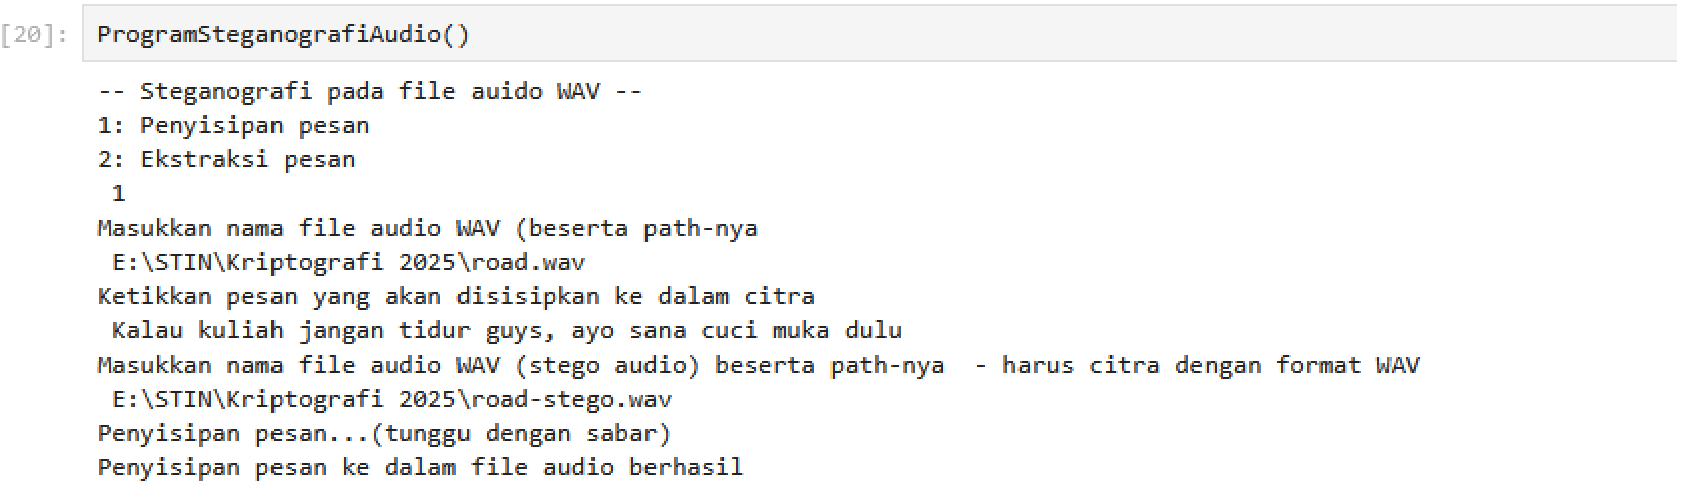
\includegraphics[width=185.01mm,height=134.24mm]{../../images/llm/page_091_img_01.png}%
\end{textblock*}

% deskripsi: Screenshot output program Python untuk ekstraksi pesan dari file audio stego WAV.
% bbox normalisasi: [0.0600, 0.5840, 0.9410, 0.9010]
\begin{textblock*}{185.01mm}(12.60mm,173.45mm)
\noindent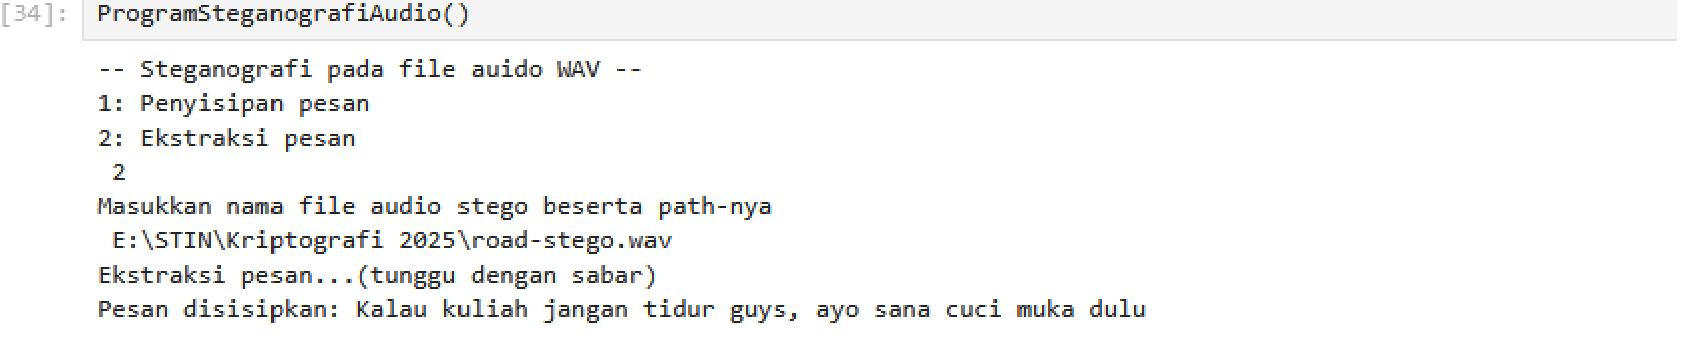
\includegraphics[width=185.01mm,height=94.15mm]{../../images/llm/page_091_img_02.png}%
\end{textblock*}

\end{document}
